\chapter{Evaluation}

\section{Functional Evaluation}
When developing the API, it is useful to already have guest code utilizing the API to quickly iterate. The following proof of concept is one of the guest programs created to test the API. It touches on all the parts of the API: getting device updates and receiving and sending data through the USB interface. As it is a proof of concept, it does not test the performance of the API.

The general idea of the program is to control a game controller. The program is started and observes the connected devices. Once a controller is connected that is recognized by the program, the program will connect to the controller. The state of all the controls of the device will be read, and input updates will be print out. To test sending data over the USB interface, the program will send commands to the controller to activate the rumble motors \footnote{Rumble motors are used to vibrate the controller}.

\subsection{Test Setup}
The code will call the event-related API to start watching for USB devices. It will get events when devices are connected or disconnected. As WASI does not support asynchronous code yet, a form of polling is used to get device connection events. The guest code uses a single-threaded asynchronous runtime, which will often yield to get new device connection events. This way, a multi-threaded real app can be simulated.

Each time a device connection event happens, the device product and vendor ID are checked to see if they match the predefined controller product and vendor ID. A Google Stadia controller is used to test this code, so the IDs of this controller type are used. If the IDs match, a connection is made to the device by opening a device handle. When a device disconnection event with matching IDs happens, the program will stop reading the controller state, and wait for a new connection.

Next, the program will try reading the controller state. This way, it knows about the positions of buttons, joysticks, triggers, etc. In order to do this, the correct interface and endpoint must be chosen. Input devices, like controllers or mice, send their data over the Interrupt transfer type, because the data sent is small and time-sensitive. Knowing this information, the interfaces can be requested and filtered to select the correct interface. In order to send information over the interface, it must first be claimed by the program. Some operating systems will attach to the interfaces by default. The host code of the API will automatically disconnect kernel attachments when claiming an interface. However, different operating systems can have different behavior in this part. For example, macOS, where the example program was ran on, does not allow detaching kernel interfaces by default for certain device classes, such as controllers. This is problematic, as we cannot interact in any way with the device this way. Elevated privileges (\texttt{sudo}) were required to get the program working. While being annoying, this was also a useful discovery, as this issue can be added to the proposal, so the standard can adjust to this.

Once the interface is claimed, device state can be requested by reading the interrupt state with the correct endpoint address. An array of bytes will be received, and by observing what changes when pressing a button, the byte layout can be decoded. A sample controller state output is showed in Code snippet \ref{code:wasi_controller_sample_output}.

\begin{code}
\begin{verbatim}

dpad: ,
buttons: assistant_button|l2_button|r2_button,
left stick: x: 128 y: 128,
right stick: x: 128 y: 128,
l2: 255,
r2: 172
\end{verbatim}
\caption{Reading controller state}
\label{code:wasi_controller_sample_output}
\end{code}

Lastly, the program also tests sending data over the USB interface. A controller is generally an input-only device. However, modern controllers often have a rumbling feature, where the controller will vibrate to get a more immersive playing experience. This program sends data over the USB interface to control the rumble feature. It will map the state of the shoulder trigger button pressure to the intensity of a rumble motor.

\subsection{Results}
This program has been tested with a Google Stadia controller. When pressing one or multiple buttons, the correct state is printed out. When pressing one or both of the shoulder buttons, the controller starts to vibrate.



\section{Performance Testing}

Tests were performed to evaluate the performance of the API. In these tests, test programs are created which run in WASI, as a native program or, when available, on Wasm in the browser. Table \ref{table:test_hardware} shows the hardware configurations of the devices used to do these tests.

\begin{table}[H]
\[
\begin{array}{|l|l|l|l|l|l|}
\hline
\textbf{Device Kind} & \textbf{Name} & \textbf{SoC/Microcontroller} & \textbf{RAM} & \textbf{Storage} \\
\hline
\text{Host} & \text{Apple Macbook Air (2020)} & \text{Apple M1 (8-core CPU, 7-core GPU)} & \text{8GB} & \text{256GB SSD} \\

\hline
\text{Guest} & \text{Arduino Micro} & \text{Atmel ATmega32U4} & \text{2,5KB} & \text{32KB Flash} \\
\hline
\end{array}
\]
\caption{The hardware used for testing the performance of the API}
\label{table:test_hardware}
\end{table}


\subsection{Latency}

One of the advantages of \acrshort{Wasm} should be that it offers near-native speed. Therefore, it is interesting to test if running a program in Wasm brings any performance overhead compared to a native program. For an USB API, this can best be tested by measuring the latency when sending or receiving data. It can be problematic if the overhead is large, as data exchange through USB happens by receiving or sending data in small chunks. Each of these chunks has to pass through the Wasm bridge and has its own overhead.

\subsubsection{Test Setup}
A program has been written with LibUSB (Native), WASI USB (Wasm) and WebUSB (Browser). Each program will do the following steps:

\begin{enumerate}
\item Enumerate the USB devices.
\item Find the Arduino board, based on its product and vendor id.
\item Open the device and claim the Bulk interface.
\item Send the \acrfull{DTR} signal to the Arduino. This signal is sent to the Arduino to acknowledge that the host device is ready to receive data. Once the Arduino has received this signal, its setup phase is completed and it will start sending data.
\item \textit{Warm up } the interface by throwing away the first batch of readings. By doing this, initial latency is removed from the measurements.
\item Read data from the Bulk interface, while measuring how long this operation takes. The arduino sends data in batches in 64 bytes, and the program will read them a million times. The program will throw away the read results, so only the transfer of the data is measured. In total, 64MB is received by the host.
\item Write durations to file.
\end{enumerate}

\subsubsection{Results}
\begin{figure}[H]
  \centering
  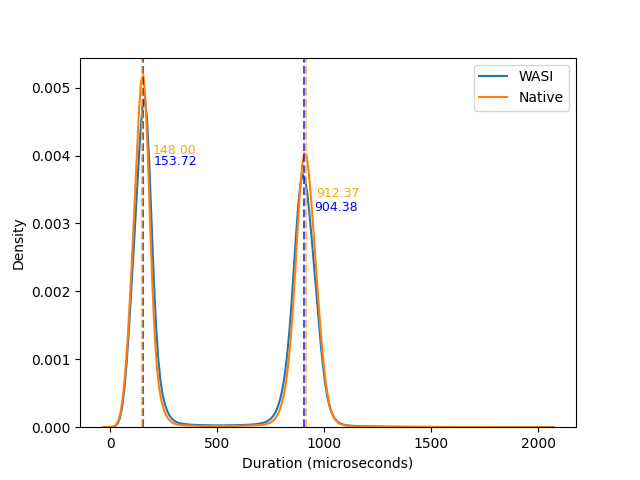
\includegraphics[width=1\textwidth]{images/reading_data_latency.png}
  \caption{Latency of reading data from Arduino using read-bulk}
  \label{fig:arduino_reading_latency}
\end{figure}


\paragraph{Interpreting Results}
Figure \ref{fig:arduino_reading_latency} shows a \acrfull{KDE} for the measurements of the native and \acrshort{WASI} implementation.
Both graphs will show peaks around the 150μs and 910μs marks. This is an interesting result, as one would expect one uniform distribution instead of two. The first peak is trivial to explain: the Arduino is an USB 2.0 device, also known as a High-speed USB device. A High-speed USB device will send frames at a fixed interval of 125μs. Therefore, we will receive new data approx. every 125μs. An extra 25μs are introduced because of processing delays.

Based on the results, we can conclude that there are no measurable differences between the different implementations of the program. However, this is mainly caused by the delay of the USB protocol. This delay vastly outweighs the delays caused by overhead of the Wasm runtime, making the Wasm overhead negligible.

However, it is possible that the delay of the USB protocol is smaller on devices more powerful than an Arduino or with a more modern USB version. With these configurations, it can be possible a small overhead for Wasm becomes visible.

In order to confirm that WASI does not add noticeable latency, a new benchmark was added which will read the contents of an USB mass storage device. The advantage of this benchmark compared to the Arduino benchmark is that it better represents real-world usage, instead of being a synthetic benchmark.

\subsubsection{Test Setup}
A program has been written which will read out the file tree of a USB device, and will read the contents of each file in the file tree. The device used is a USB 2.0 Mass Storage device, which has been formatted to use the MBR partition map and the EXFat file system. Communication with the device happens over the SCSI interface. The program uses a EXFat package, which uses a generic interface which works similar to a file handle to communicate with the USB device. A SCSI adapter has been written which will read blocks of the USB device. A cache is used to simulate typical behavior of a USB mass storage driver.

An overview of the file tree of the USB device is the following:


\subsection{Memory Usage}
 